%\documentclass{standalone}
\documentclass[16pt]{article}
\usepackage{tikz}
\usetikzlibrary{decorations.pathreplacing}
\usepackage{colortbl}
%\documentclass{minimal}
%\usepackage[active,tightpage,displaymath]{preview}
%\documentclass{article}
\usepackage{blkarray}
\usepackage{amsmath}
\pagestyle{empty}
\usepackage[paperheight=16cm,paperwidth=33cm]{geometry}
%\usepackage[absolute]{textpos}

\definecolor{c1}{RGB}{102,194,165}
\definecolor{c2}{RGB}{252,141,98}
\definecolor{c3}{RGB}{141,160,203}
\definecolor{c4}{RGB}{231,138,195}

\newcolumntype{a}{>{\columncolor{LightYellow}}l}
\newcolumntype{b}{>{\columncolor{LightYellow}}c}
\newcolumntype{d}{>{\columncolor{LightGrey}}l}
\newcolumntype{e}{>{\columncolor{LightGrey}}c}

\begin{document}
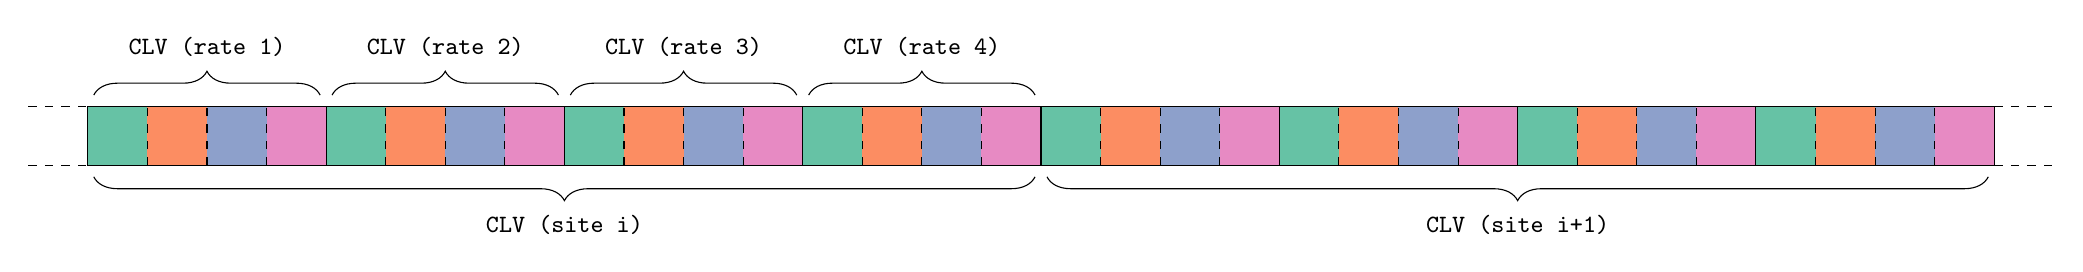
\begin{tikzpicture}[font=\small]
%\draw[step=20ex,gray,very thin] (0ex,0ex) grid (160ex,5ex);

%%% First quadruple of colors 
\fill[c1] (0ex,5ex) rectangle (5ex,0ex);
\fill[c2] (5ex,5ex) rectangle (10ex,0ex);
\fill[c3] (10ex,5ex) rectangle (15ex,0ex);
\fill[c4] (15ex,5ex) rectangle (20ex,0ex);


%%% Second quadruple of colors 
\fill[c1] (20ex,5ex) rectangle (25ex,0ex);
\fill[c2] (25ex,5ex) rectangle (30ex,0ex);
\fill[c3] (30ex,5ex) rectangle (35ex,0ex);
\fill[c4] (35ex,5ex) rectangle (40ex,0ex);

%%% Third quadruple of colors 
\fill[c1] (40ex,5ex) rectangle (45ex,0ex);
\fill[c2] (45ex,5ex) rectangle (50ex,0ex);
\fill[c3] (50ex,5ex) rectangle (55ex,0ex);
\fill[c4] (55ex,5ex) rectangle (60ex,0ex);

%%% Fourth quadruple of colors 
\fill[c1] (60ex,5ex) rectangle (65ex,0ex);
\fill[c2] (65ex,5ex) rectangle (70ex,0ex);
\fill[c3] (70ex,5ex) rectangle (75ex,0ex);
\fill[c4] (75ex,5ex) rectangle (80ex,0ex);

%%% Fifth quadruple of colors 
\fill[c1] (80ex,5ex) rectangle (85ex,0ex);
\fill[c2] (85ex,5ex) rectangle (90ex,0ex);
\fill[c3] (90ex,5ex) rectangle (95ex,0ex);
\fill[c4] (95ex,5ex) rectangle (100ex,0ex);

%%% Sixth quadruple of colors 
\fill[c1] (100ex,5ex) rectangle (105ex,0ex);
\fill[c2] (105ex,5ex) rectangle (110ex,0ex);
\fill[c3] (110ex,5ex) rectangle (115ex,0ex);
\fill[c4] (115ex,5ex) rectangle (120ex,0ex);

%%% Seventh quadruple of colors 
\fill[c1] (120ex,5ex) rectangle (125ex,0ex);
\fill[c2] (125ex,5ex) rectangle (130ex,0ex);
\fill[c3] (130ex,5ex) rectangle (135ex,0ex);
\fill[c4] (135ex,5ex) rectangle (140ex,0ex);

%%% Eigth quadruple of colors 
\fill[c1] (140ex,5ex) rectangle (145ex,0ex);
\fill[c2] (145ex,5ex) rectangle (150ex,0ex);
\fill[c3] (150ex,5ex) rectangle (155ex,0ex);
\fill[c4] (155ex,5ex) rectangle (160ex,0ex);

\draw (0ex,0ex) -- (160ex,0ex) -- (160ex,5ex) -- (0ex,5ex) -- (0ex,0ex);

\draw (20ex,0ex) -- (20ex,5ex);
\draw[dashed] (5ex,0ex) -- (5ex,5ex);
\draw[dashed] (10ex,0ex) -- (10ex,5ex);
\draw[dashed] (15ex,0ex) -- (15ex,5ex);

\draw (40ex,0ex) -- (40ex,5ex);
\draw[dashed] (25ex,0ex) -- (25ex,5ex);
\draw[dashed] (30ex,0ex) -- (30ex,5ex);
\draw[dashed] (35ex,0ex) -- (35ex,5ex);

\draw (60ex,0ex) -- (60ex,5ex);
\draw[dashed] (45ex,0ex) -- (45ex,5ex);
\draw[dashed] (50ex,0ex) -- (50ex,5ex);
\draw[dashed] (55ex,0ex) -- (55ex,5ex);

\draw (80ex,0ex) -- (80ex,5ex);
\draw[dashed] (65ex,0ex) -- (65ex,5ex);
\draw[dashed] (70ex,0ex) -- (70ex,5ex);
\draw[dashed] (75ex,0ex) -- (75ex,5ex);

\draw (100ex,0ex) -- (100ex,5ex);
\draw[dashed] (85ex,0ex) -- (85ex,5ex);
\draw[dashed] (90ex,0ex) -- (90ex,5ex);
\draw[dashed] (95ex,0ex) -- (95ex,5ex);

\draw (120ex,0ex) -- (120ex,5ex);
\draw[dashed] (105ex,0ex) -- (105ex,5ex);
\draw[dashed] (110ex,0ex) -- (110ex,5ex);
\draw[dashed] (115ex,0ex) -- (115ex,5ex);

\draw (140ex,0ex) -- (140ex,5ex);
\draw[dashed] (125ex,0ex) -- (125ex,5ex);
\draw[dashed] (130ex,0ex) -- (130ex,5ex);
\draw[dashed] (135ex,0ex) -- (135ex,5ex);

\draw[dashed] (145ex,0ex) -- (145ex,5ex);
\draw[dashed] (150ex,0ex) -- (150ex,5ex);
\draw[dashed] (155ex,0ex) -- (155ex,5ex);

\draw[decorate,decoration={brace,amplitude=2ex,raise=4pt},yshift=0pt] (0.5ex, 5ex) -- (19.5ex,5ex);
\draw[decorate,decoration={brace,amplitude=2ex,raise=4pt},yshift=0pt] (20.5ex, 5ex) -- (39.5ex,5ex);
\draw[decorate,decoration={brace,amplitude=2ex,raise=4pt},yshift=0pt] (40.5ex, 5ex) -- (59.5ex,5ex);
\draw[decorate,decoration={brace,amplitude=2ex,raise=4pt},yshift=0pt] (60.5ex, 5ex) -- (79.5ex,5ex);
\node at (10ex,10ex) {\tt CLV (rate 1)};
\node at (30ex,10ex) {\tt CLV (rate 2)};
\node at (50ex,10ex) {\tt CLV (rate 3)};
\node at (70ex,10ex) {\tt CLV (rate 4)};
\draw[decorate,decoration={brace,amplitude=2ex,mirror,raise=4pt},yshift=0pt] (0.5ex, 0ex) -- (79.5ex,0ex);
\node at (40ex,-5ex) {\tt CLV (site i)};
\draw[decorate,decoration={brace,amplitude=2ex,mirror,raise=4pt},yshift=0pt] (80.5ex, 0ex) -- (159.5ex,0ex);
\node at (120ex,-5ex) {\tt CLV (site i+1)};

\draw[dashed] (-5ex,0ex) -- (0ex,0ex);
\draw[dashed] (-5ex,5ex) -- (0ex,5ex);
\draw[dashed] (160ex,5ex) -- (165ex,5ex);
\draw[dashed] (160ex,0ex) -- (165ex,0ex);
\end{tikzpicture}
\end{document}
